\subsection{Główna struktura interfejsu}

Przygotowano interfejs zgodnie z ustalonymi wymaganiami. W celu ułatwienia pracy
w wielu edytorach w tym samym czasie, zaimplementowano system kart.
Zaimplementowano możliwość przełączania motywu aplikacji z jasnego na ciemny i
odwrotnie. Główny interfejs zamieszczono na rysunku \ref{mainInterfaceFigure}.

Aplikacja frontend została zaprojektowana w sposób typowy dla aplikacji SPA
\cite{mikowski2013single} z wykorzystaniem biblioteki React.js. Aplikacja nie
wymaga ładowania nowej strony przez przeglądarkę podczas pracy.

Składa się z komponentów, z których niektóre są używane w wielu miejscach
aplikacji. Komponenty, które implementują skomplikowaną funkcjonalność zawierają
komponenty podrzędne.

Główny komponent aplikacji to widok kart (\verb|TabsView|). Komponent zawiera
pasek kart (\verb|TabBar|) oraz komponent służący do wybierania edytorów
(\verb|EditorSelector|). Komponent \verb|TabBar| implementuje listę kart, która
pozwala użytkownikowi na przełączanie się pomiędzy edytorami. Karty, które nie
są aktywne są chowane za pomocą ustawienia wartości CSS \verb|display| na
\verb|none|. W ten sposób, nie tracą danych przechowywanych w stanie komponentu
przy przełączaniu kart. Komponent \verb|EditorSelector| pozwala na wybór
edytora. Edytory zawierają interfejs, przy użyciu którego administrator wykonuje
pracę na systemie CMS.

Komponent \verb|EditorSelector| pobiera dane o dostępnych edytorach ze struktury
danych. Umożliwia to łatwe dodawanie nowych edytorów do aplikacji. Strukturę
danych widać na listingu \ref{editorListListing}. Struktura danych przechowuje
dane o folderach, które mogą zawierać edytory. Foldery i edytory mają ikonę oraz
opis, a edytory mają również komponent. Przy wyborze edytora, komponent
przypisany do tego edytora zostanie wyświetlony na ekranie.

\lstinputlisting[
    float=h!,
    frame=tb,
    label={editorListListing},
    caption={Struktura danych przechowująca dane o edytorach}
]{./code/editors.ts}

Aplikacja frontend pozwala użytkownikowi na zmianę motywu. Użytkownik może
wybrać motyw jasny i ciemny. Przełączenie motywu powoduje podmienienie zmiennych
CSS z kodu aplikacji. Wybrany przez użytkownika motyw jest zapisywany z
wykorzystaniem standardowej funkcji przeglądarki \verb|localStorage| i ładowany
przy uruchomieniu aplikacji. Domyślny motyw to motyw jasny (ciemny tekst na
jasnym tle). Kod odpowiedzialny za przełączanie motywu został zamieszczony na listingu
\ref{schemeTogglingListing}.

\lstinputlisting[
    float=h!,
    frame=tb,
    label={schemeTogglingListing},
    caption={Kod odpowiedzialny za przełączanie motywu}
]{./code/schemeToggling.ts}


\begin{figure}
    \centering
    \subfloat[\centering Motyw jasny]
        {{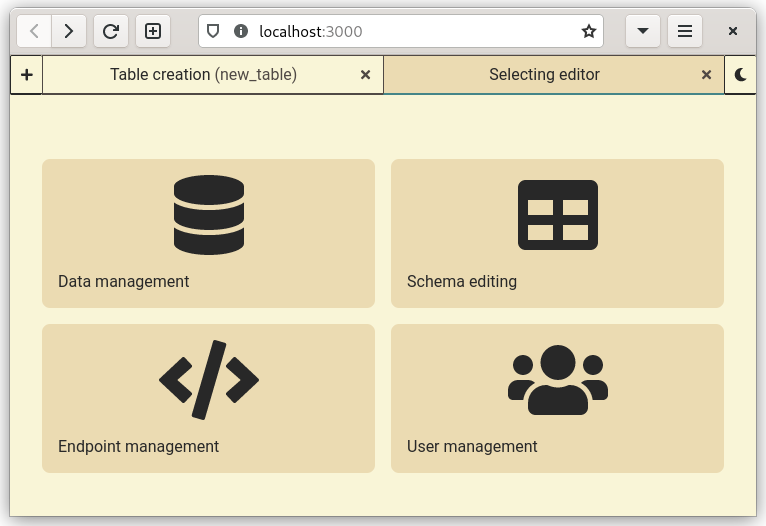
\includegraphics[width=.45\linewidth]{./img/starting_view_light.png} }}
    \qquad
    \subfloat[\centering Motyw ciemny]
        {{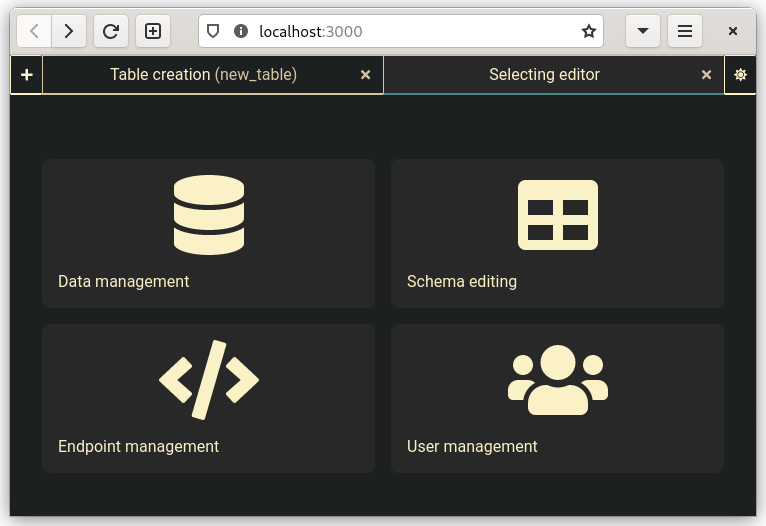
\includegraphics[width=.45\linewidth]{./img/starting_view_dark.png} }}

    \caption{Główny interfejs aplikacji}
    \label{mainInterfaceFigure}
\end{figure}

